\documentclass{bioinfo}

\usepackage{subfigure}

\copyrightyear{2010}
\pubyear{2010}

\begin{document}
\begin{application}
\firstpage{1}

\title[SMM Project]{Stabilization matrix method - Mini project}
\author[Sigmar Stefansson, Francesco Favero]{Sigmar Stefansson and Francesco Favero}
\address{Danmarks Tekniske Univeristet}

\history{22 October 2010}

\editor{Supervisor: Morten Nielsen}

\maketitle

\begin{abstract}

\section{Summary}
We look at Stabilization matrix methods using two different kinds of minimizations procedures \cite{SMM} for predicting binding \cite{netMHC} affinity of immunogenic peptides to major histocompatibility complex \cite{wiki:MHC} (MHC) molecules.
\par The testing data available was from 35 different MHC molecules from HLA-A and HLA-B, with number of peptides ranging from 59 to 3089.
\par Finally we studied the results of the Monte Carlo and the gradient decent implementations of the SMM, to find the optimal setting of the algorithms.

\end{abstract}

\section*{Introduction}

In simple mathematical terms the SMM algorithm tries to minimize the difference between the predicted values and the measured values according to a norm.

\begin{equation}
\label{eq:01}
\| H w - y_{meas}\| + ^tw \Lambda w \rightarrow minimum \\
\end{equation}

In this case the L2 norm is used. The second term suppresses the effect of noise in the experimental data \cite{SMM}. The regulation parameter $\lambda$ is used to deal with over-fitting in the SMM algorithms \cite{wiki:overfit}. In the context of the SMM algorithm, H is a matrix encoding the peptides, w is the prediction (position specific scoring) matrix and $y_{meas}$ is vector containing the measured binding affinity of the peptides.

\par Over-fitting occurs when a statistical model describes random error or noise instead of the underlying relationship \cite{Hobohm}. A model having too many degrees of freedom, in relation to the amount of data available is susceptible to over-fitting. A model which has been overfit will generally have poor predictive performance. Among common methods of avoiding over-fitting are early stopping and cross-validation.
\par In early stopping, the training is stopped based on test set performance (when it starts decaying). Cross-validation is about combining models. In K-fold cross-validation, the original sample is randomly partitioned into K sub samples. Of the K sub samples, a single sub sample is retained as the validation data for testing the model, and the remaining K − 1 sub samples are used as training data. The cross-validation process is then repeated K times (the folds), with each of the K sub samples used exactly once as the validation data \cite{wiki:crossval}.
\par In terms of the SMM algorithm, the solution is not found by simple matrix inversion using \ref{eq:01}. The system of linear equations is under- or overdetermined and an approximate solution is to be located on the solution hyper-surface that can contain local minima. Equation \ref{eq:02} shows how the error used in the minimization procedure is calculated. O and t being the prediction output and the measurement respectively.

\begin{equation}
\label{eq:02}
E = \frac{1}{2} \sum_i{(O_i-t_i)^2} + \lambda \sum_l{w_i^2} \\
\end{equation}


\section*{Material and Methods}

We were given semi-completed code for the implementation of the Stabilization matrix method. The minimization procedures were Gradient descent in one case and Monte Carlo in the other. 
\par The testing data available was from 35 different MHC molecules from HLA-A and HLA-B, with number of peptides ranging from 59 to 3089. In addition to finishing the code we added some optimizations like skipping unnecessary memory allocations at performance critical locations.
<<<<<<< HEAD
\par We ran the matrix creation on each 35 MHC molecules to get the broadest perspective. The code did run fast enough for us to be able to search for optimal $\lambda$ value with brute force. The $\lambda$ values we tested were 0, 0.002, 0.005, 0.01, 0.02, 0.03, 0.05 and 0.1. For largest data sets the optimal lambda values were the ones close to zero, 0.002 and 0.005.
\par Regardless the size of the data, for the two implementations the optimal value of $\lambda$ is different. In Figure \ref{fig:07} all the 35 Pearson correlation coefficient are include. As we can see the Monte Carlo is better with smaller value of $\lambda$ (around 0.005 and 0.01), the gradient decent version have the optimal $\lambda$ value slightly bigger( best $\lambda$ around 0.02).
=======
\par We ran the matrix creation on each 35 MHC molecules to get the broadest perspective. The code did run fast enough for us to be able to search for optimal $\lambda$ value by brute force. The $\lambda$ values we tested were 0, 0.002, 0.005, 0.01, 0.02, 0.03, 0.05 and 0.1. For the largest data sets the optimal lambda values were the ones close to zero, 0.002 and 0.005.
\par Regardless the size of the data, for the two implementations the optimal value of $\lambda$ is different. In Figure \ref{fig:07} all the 35 Pearson correlation coefficents are included. As we can see the Monte Carlo is better with smaller value of $\lambda$ (around 0.005 and 0.01), the gradient decent version have a slightly larger optimal $\lambda$ value (best $\lambda$ around 0.002) see Figure \ref{fig:02}.
>>>>>>> 531bfa3650e2ec3ff96a3c0e958b3417a908f8e5

\begin{figure}[!tpb]
\begin{center}
\subfigure[Gradient decent]{
	\label{fig:08}
	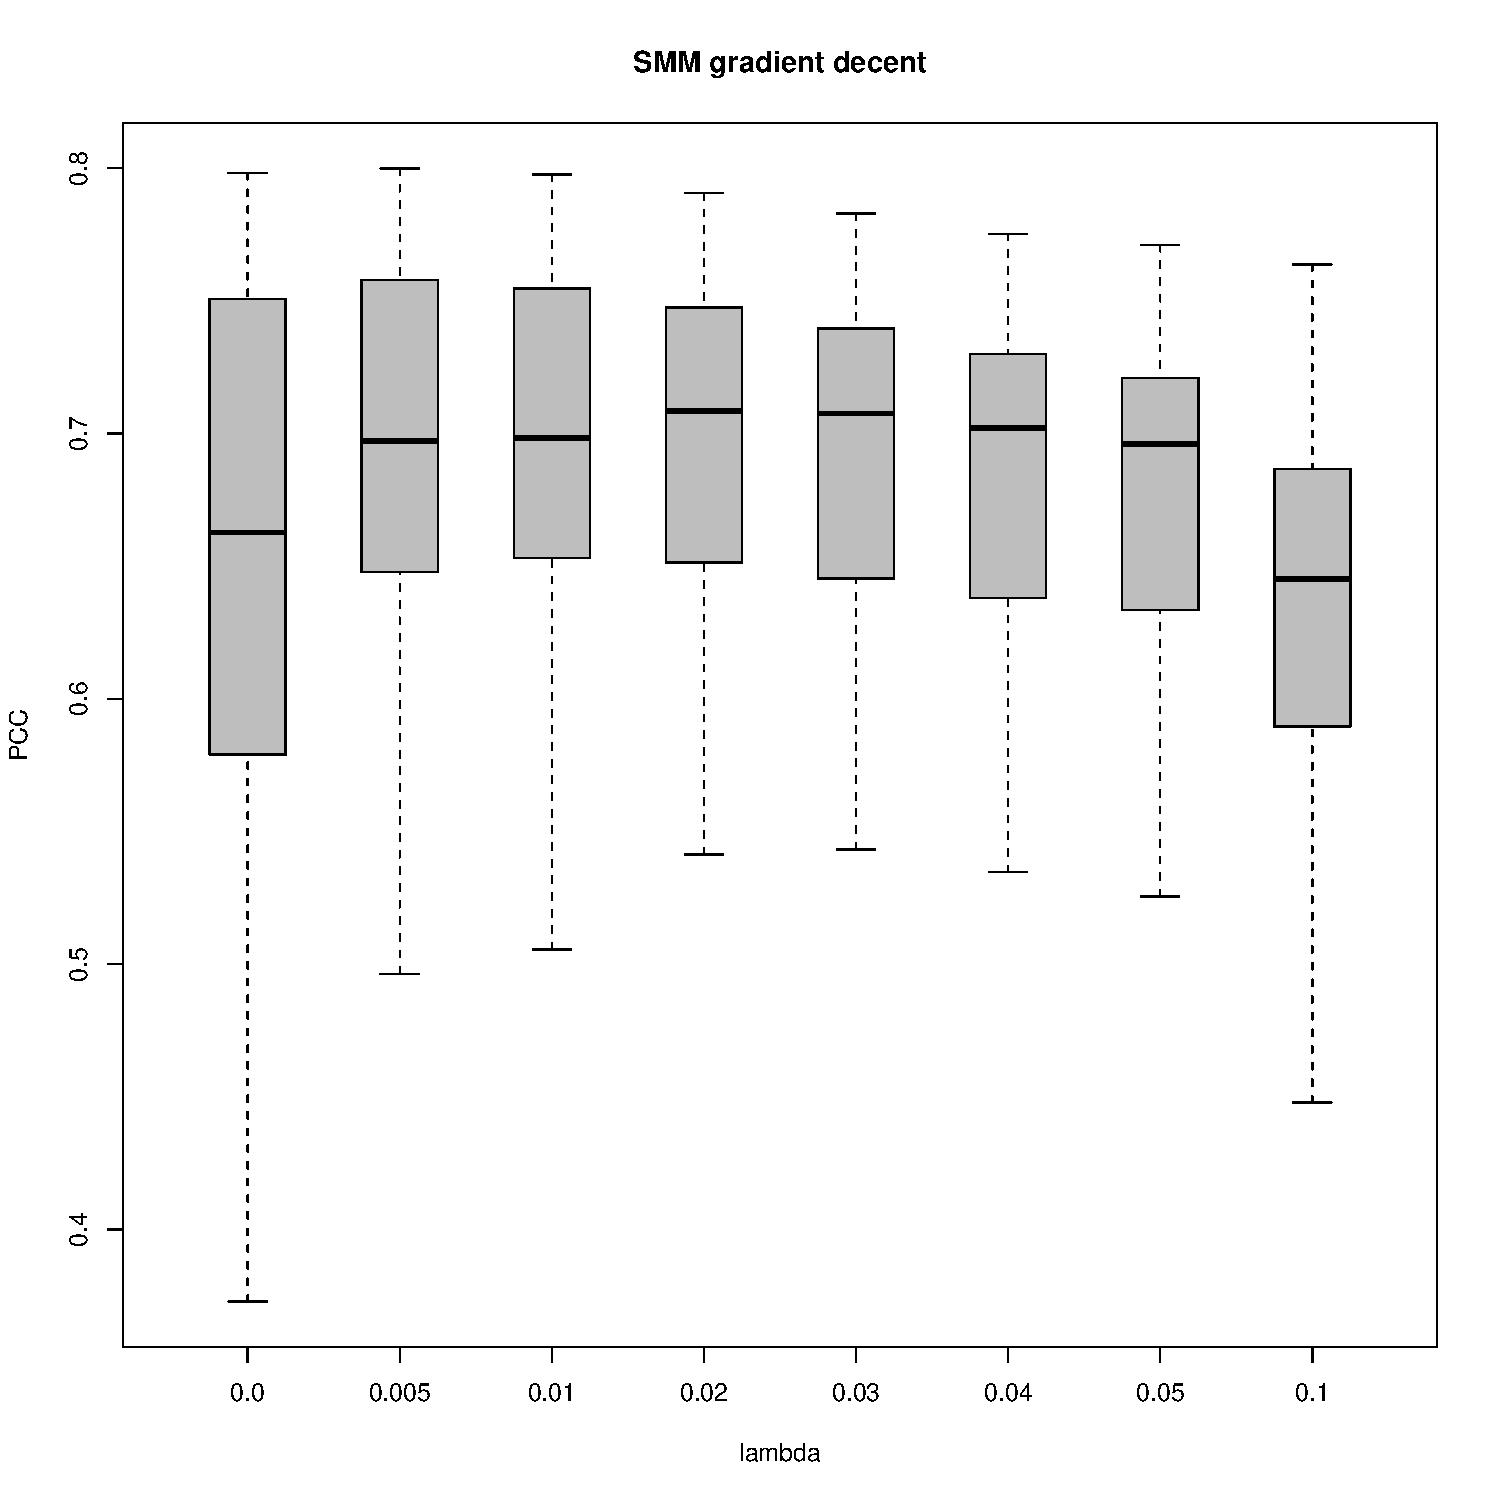
\includegraphics[width=4cm]{fig/choice_lambda.pdf}
	}
\subfigure[Monte Carlo]{
	\label{fig:09}
	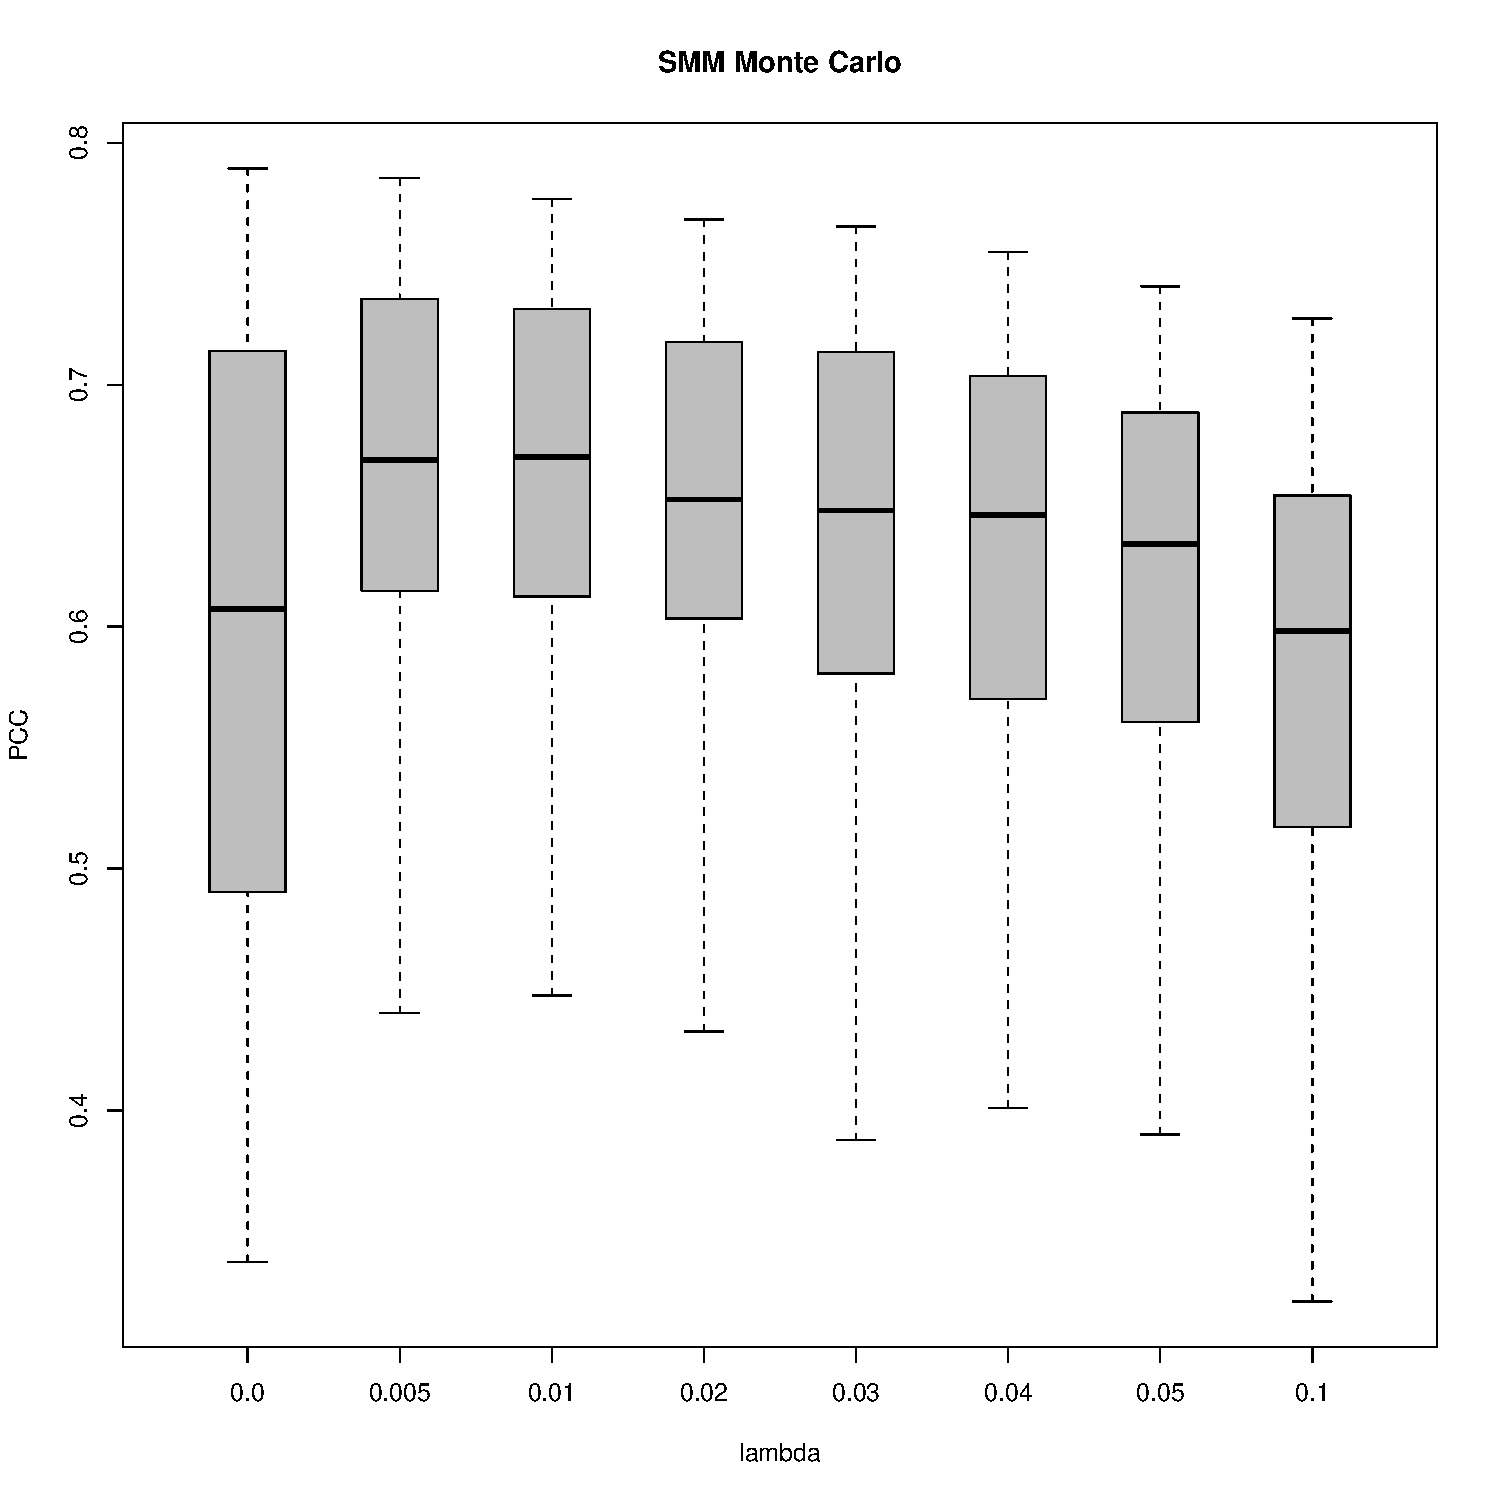
\includegraphics[width=4cm]{fig/choice_lambda_mc.pdf}
	}
\end{center}
\caption{Plot of Pearson correlation coefficients at progressive increasing of $\lambda$ values, for the gradient decent \ref{fig:08} and for the Monte Carlo \ref{fig:09} implementation}
\label{fig:07}
\end{figure}

\par The data for each MHC molecule was splitted into five parts, equally (or nearly equally) sized. Each part was then used for the validation by the K-fold cross validation method \cite{wiki:crossval}. So each part was trained on the rest (4/5) of the data, resulting in 5 iterations to be used for the evaluation.
\begin{figure}[!tpb]
\centerline{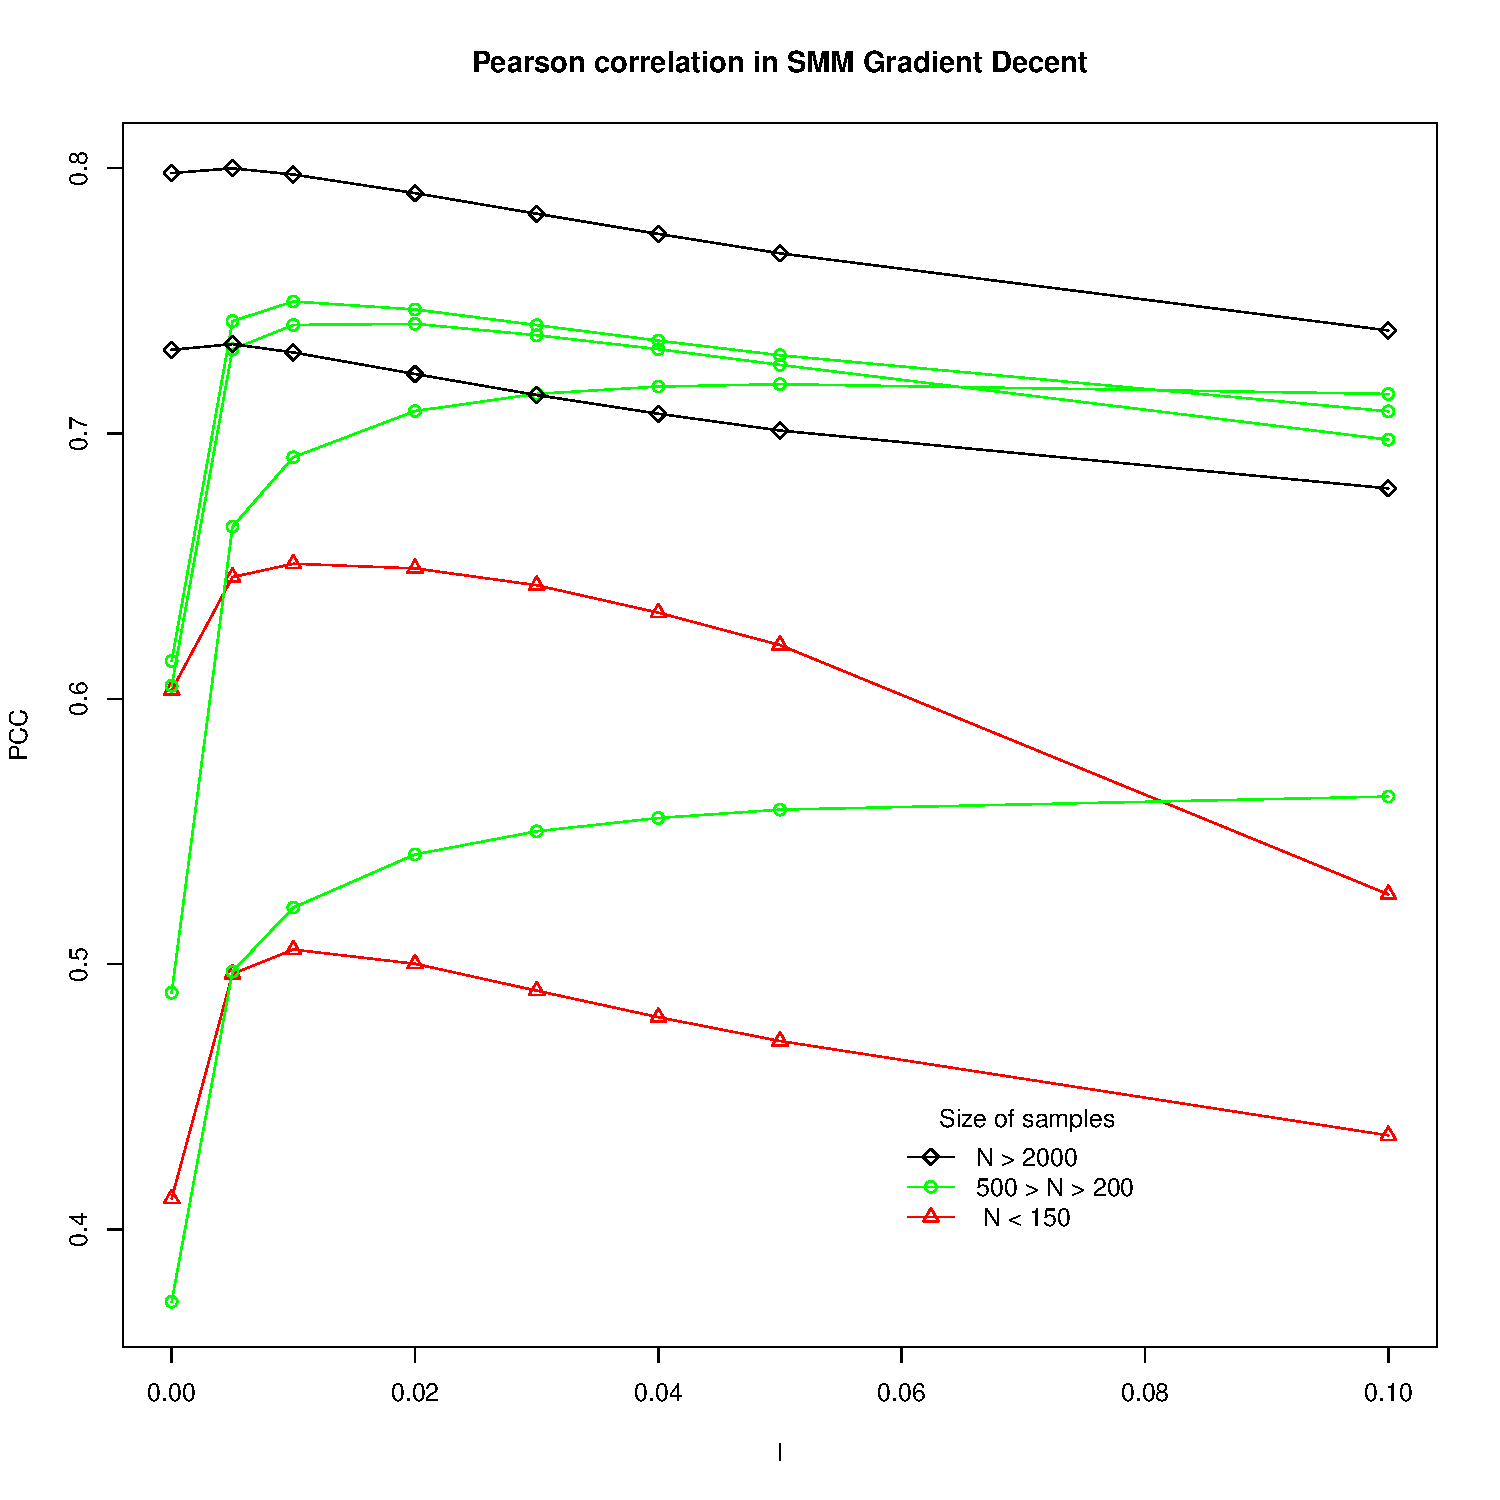
\includegraphics[width=9cm]{fig/smm_l005_ppc_size.pdf}}
\caption{Pearson's correlation coefficient  from the SMM Gradient Decent,of different sample using increasing values of $\lambda$. The sample were grouped by the size of the dataset. We can see how dataset of similar size show a similar trend of the Pearson correlation $\lambda$ depending.}
\label{fig:01}
\end{figure}

\par In order to find the optimal $\lambda$ value we evaluate the correlation of all the 35 molecules with both algorithms with different $\lambda$ parameter. To reduce the running time of the procedure we splitted the list of the 35 dataset in 7 different jobs taking care of 5 dataset each. 
\par As noted in Figure \ref{fig:01} and in Figure \ref{fig:02} the use of the $\lambda$ value suppresses the effect of noise in the measured data. In the case of zero value $\lambda$, the optimal entries for the weight vector \textit{w} minimize the difference between predicted and measured values.  Minimizing with a non-zero value for $\lambda$ results in a shift of the optimal entries in \textit{w} towards values closer to zero. It should be noted here that the $\lambda$ value used as a parameter in the code is the per-target normalized $\lambda$ value, not the global one.

\begin{figure}[!tpb]
\centerline{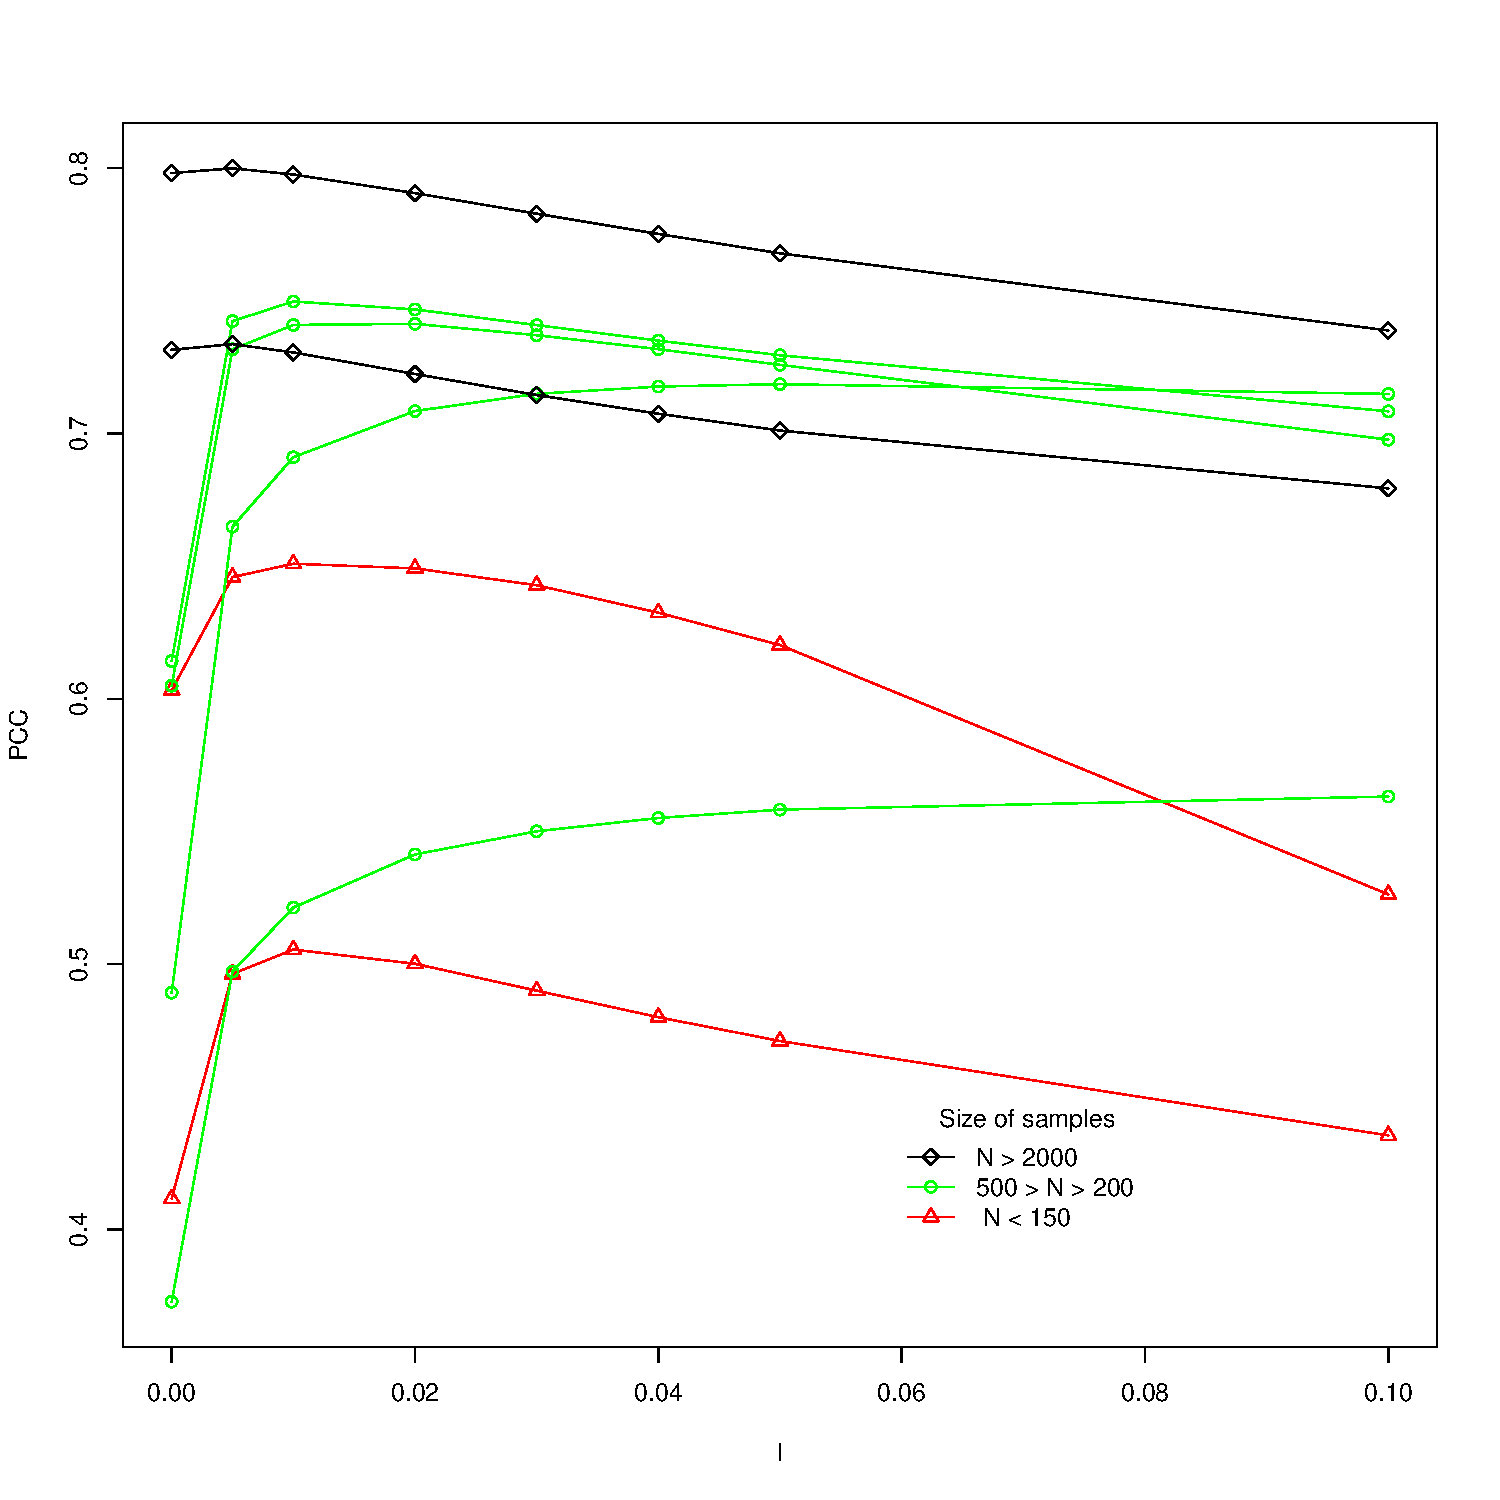
\includegraphics[width=9cm]{fig/smm_mc_l005_ppc_size.pdf}}
\caption{Pearson's correlation coefficient from the SMM Monte Carlo, of different sample using increasing values of $\lambda$. The sample were grouped by the size of the dataset. We can see how dataset of similar size show a similar trend of the Pearson correlation $\lambda$ depending.}
\label{fig:02}
\end{figure}
\par We also evaluate each single group of peptide binding data. From the bar-plot in Figure \ref{fig:05} we can see how the 5-fold concatenate evaluation it is not better than all the single fold evaluation, but it is seems more an average of all them.

\begin{figure}[!tpb]
\centerline{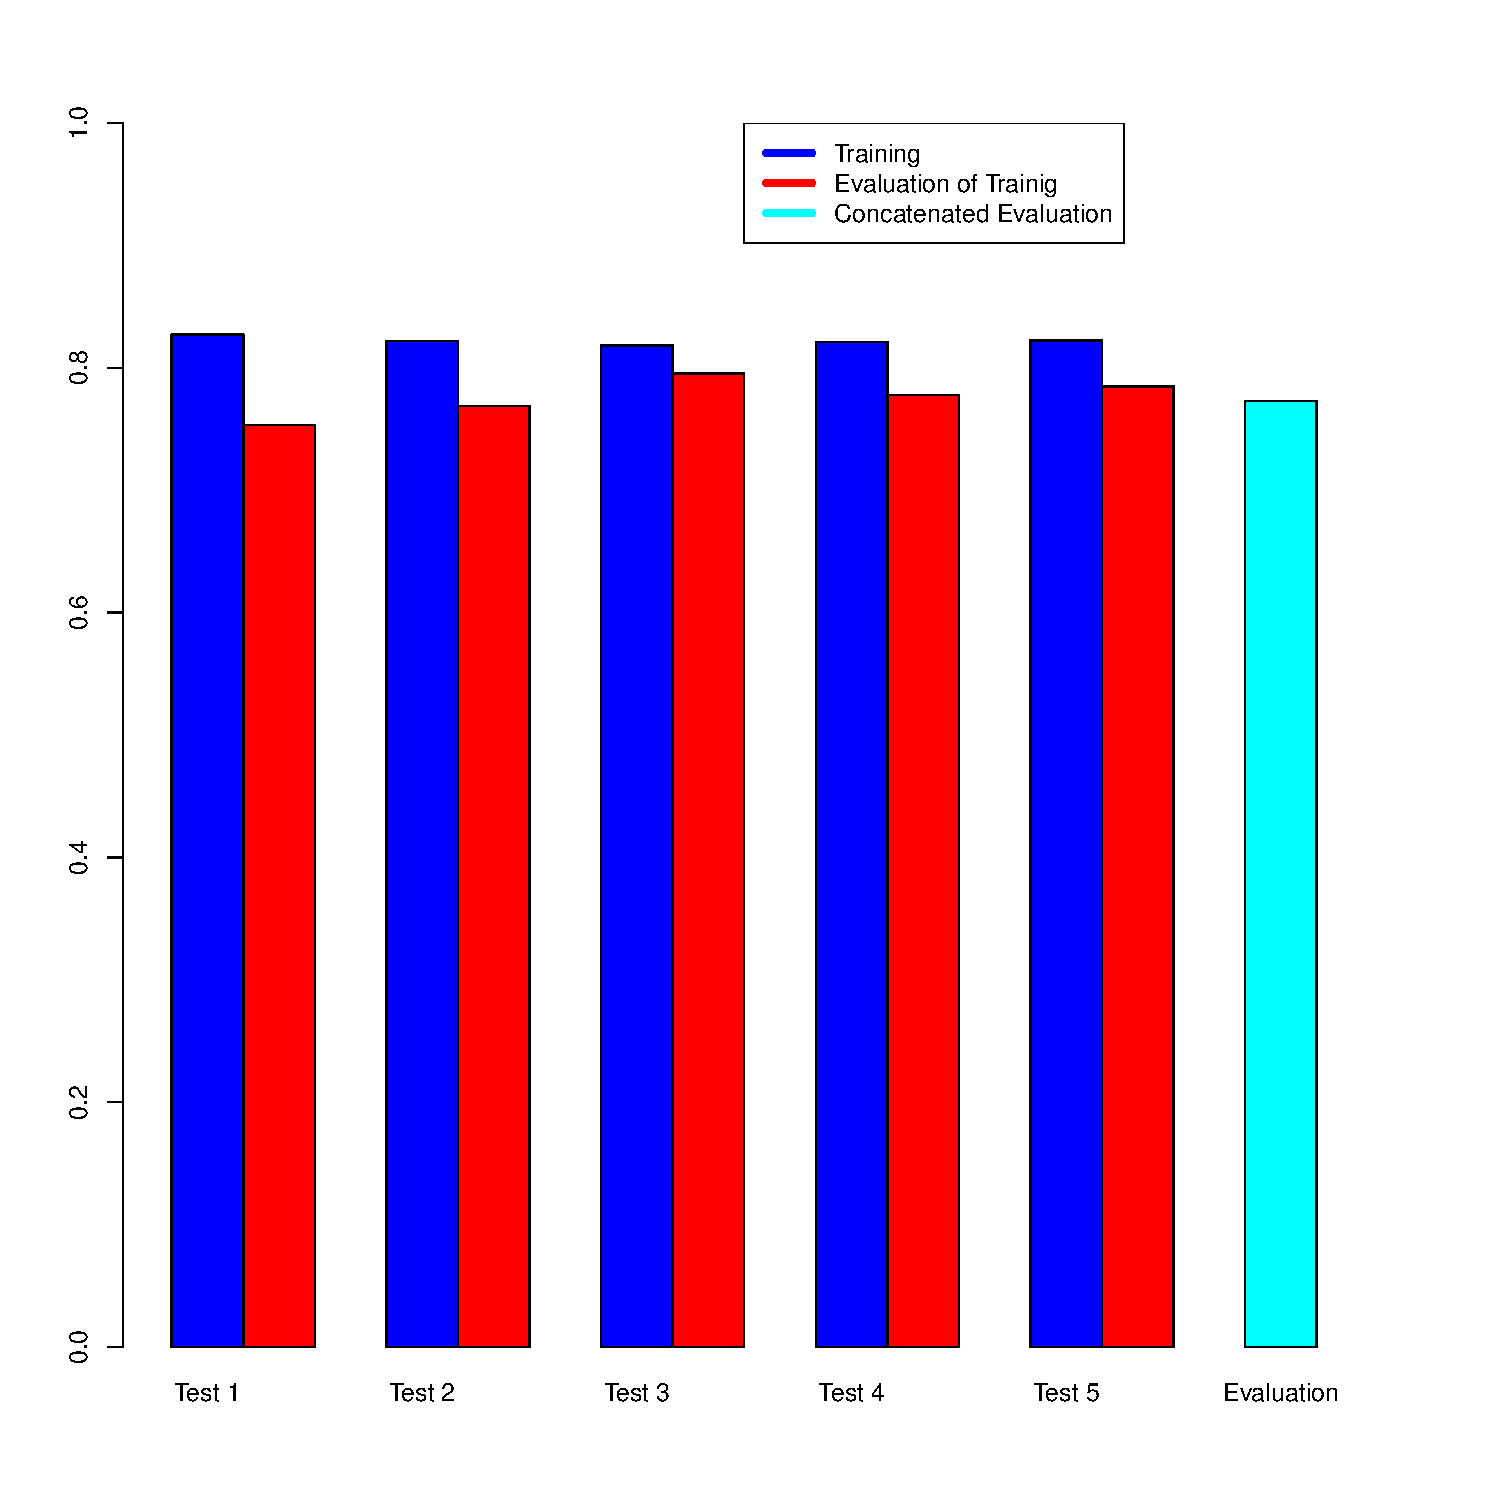
\includegraphics[width=9cm]{fig/barplot.pdf}}
\caption{Bar-plot showing the Pearson Correlation for each training set, for each evaluation on the test set and the correlation of the concatenate evaluation among the 5 test set}
\label{fig:05}
\end{figure}



\section*{Results}

\begin{figure}[!tpb]
\centerline{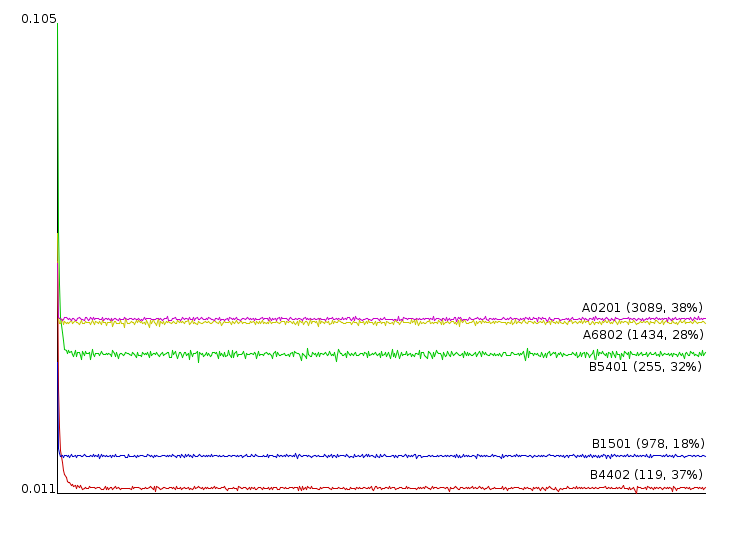
\includegraphics[width=9cm]{fig/smm_error.png}}
\caption{Error trend for dataset of different size in function of the number of cycle of the SMM gradient decent algorithm}
\label{fig:03}
\end{figure}

Figure \ref{fig:01} shows the trend for Pearson's correlation coefficient (PCC, prediction accuracy) using different $\lambda$ values for various data sizes.




\begin{figure}[!tpb]
\centerline{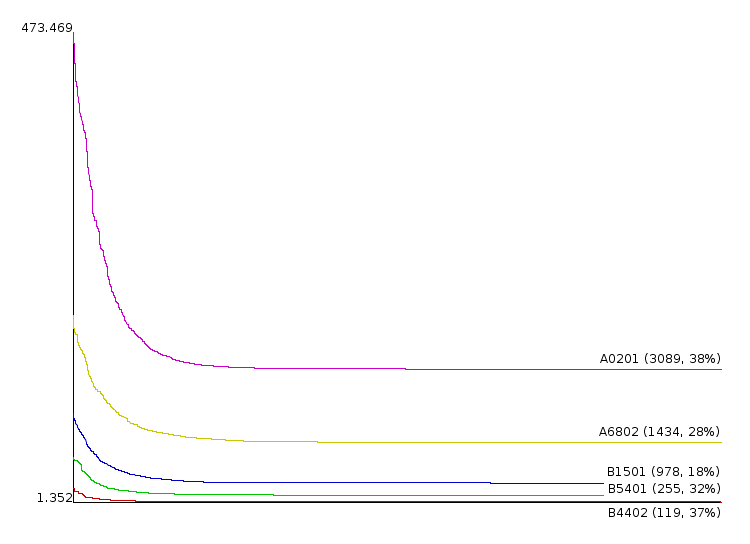
\includegraphics[width=9cm]{fig/smm_mc_error.png}}
\caption{Error trend for dataset of different size in function of the number of cycle of the SMM Monte Carlo algorithm}
\label{fig:04}
\end{figure}

\par As a general rule, as the data size gets larger the less important the effect of a non-zero $\lambda$ becomes. For large data sets a $\lambda$ value of zero seems to give the best results. A large dataset should average out the noise. Similar graph showing results from the Monte Carlo version says the same story (Figure \ref{fig:02}).
\par For the small datasets an optimal $\lambda$ value is  less than 0.01. Next we run the SMM algorithms on a data from five different kinds of MHC molecules (with different data sizes) showing the error as a function of iterations. For the SMM algorithm using gradient descent and 500 iterations, a default lambda value of 0.05 is used (Figure \ref{fig:03}). Similar chart is shown for the Monte Carlo version of the algorithm in Figure \ref{fig:04} showing 12000 iterations. The reason for showing different data sizes on the same chart is just for showing the trends in the two different algorithms. The gradient descent method converges much faster to an optimal value than the Monte Carlo method. The data sizes and percentage of number of binding peptides are shown in the parentheses right by the names of the lines representing each MHC molecule.

\par The gradient descent version of the SMM algorithm is both performing faster and better than the Monte Carlo version. The speed of the convergence is determined by the derived slope in gradient descent. The Monte Carlo version lowers the temperature not in the context of a slope.
\begin{figure}[!tpb]
\centerline{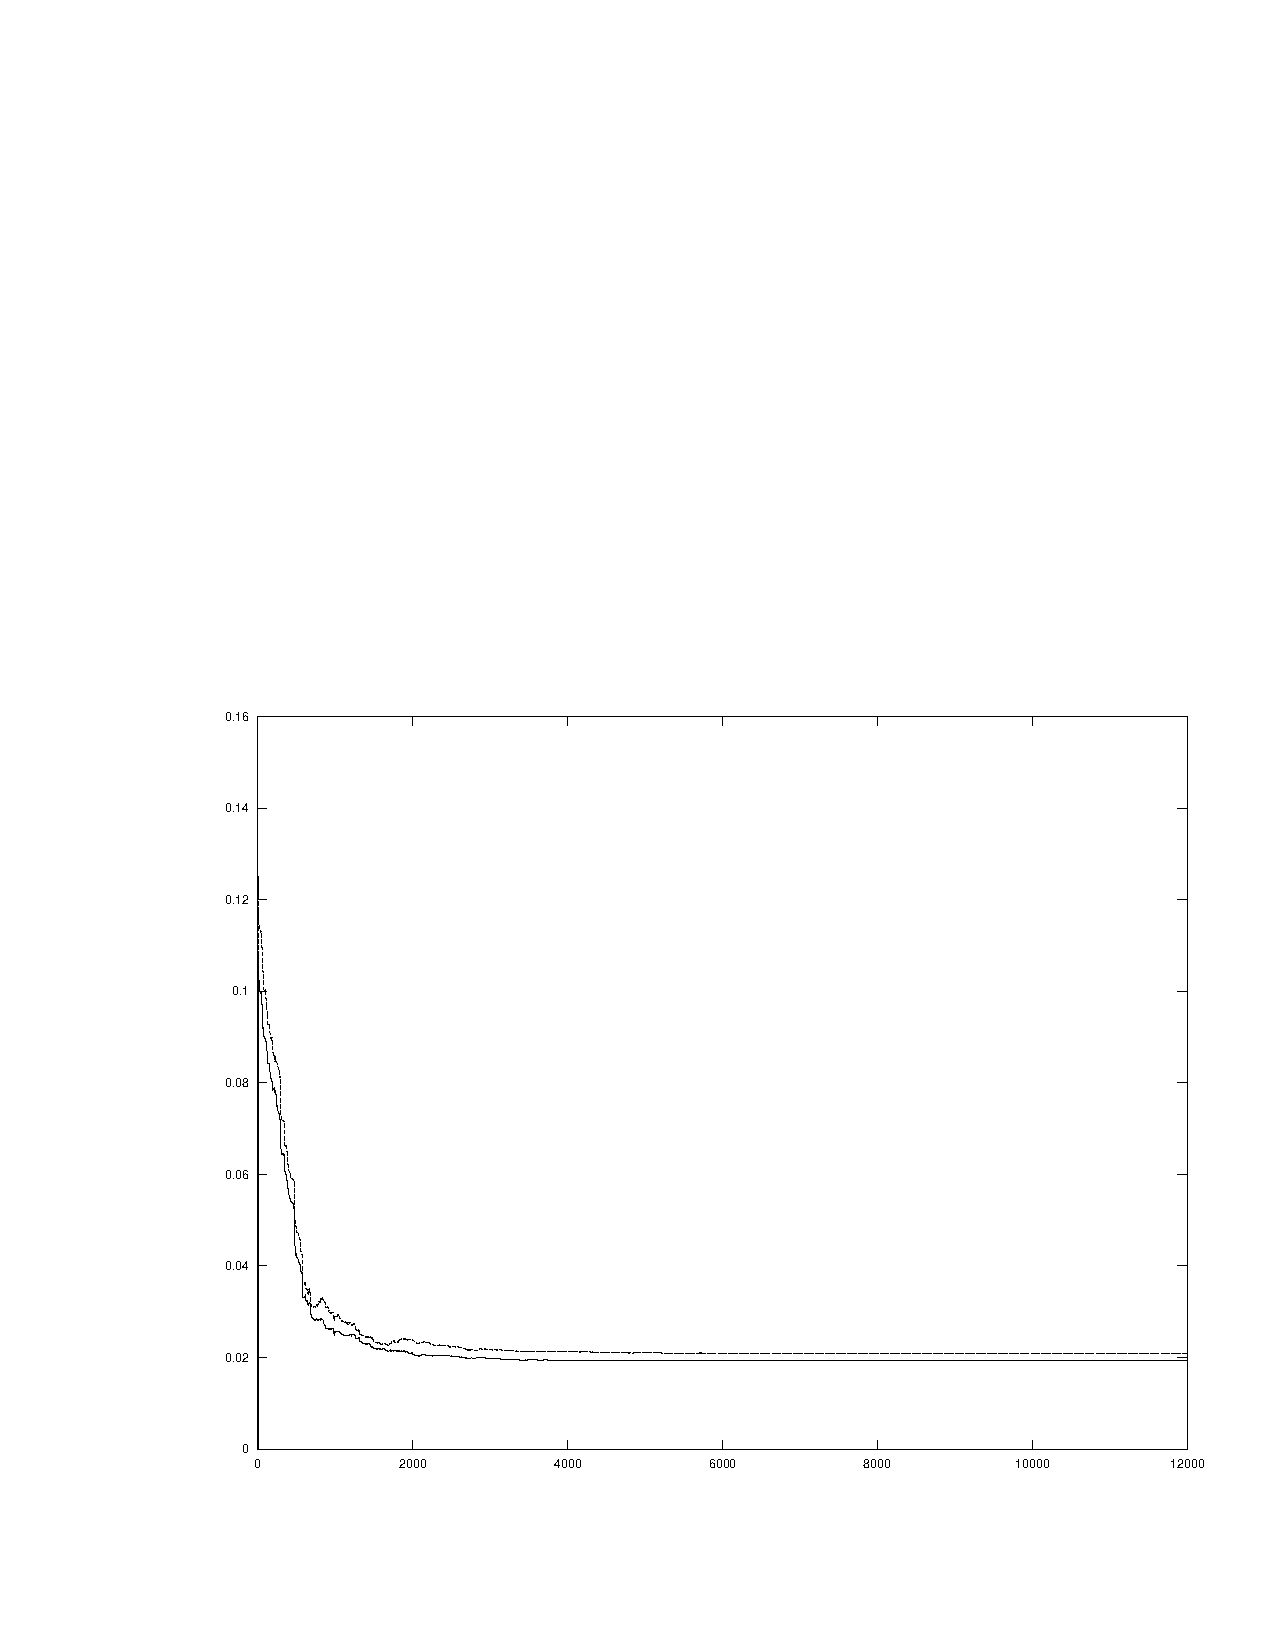
\includegraphics[width=9cm]{overfitting_not.pdf}}
\caption{When training the Monte Carlo version of the algorithm with a $\lambda$ of 0.05, the mean square error for the testing seems to follow the training error pretty well. In this case an early stopping to prevent overfitting is unnecessary}
\label{fig:05}
\end{figure}

\par We made some adjustments to the c code to be able to compare the mean square error (MSE) of the training and testing results in each cycle. The gradient descent version converged in most cases in just one or two iterations. In Monte Carlo the testing MSE did not seem to decay with continuing iterations, indicating that preventing overfitting with early stopping would not be practical in that case \ref{fig:05}.



\section*{Discussion}



\begin{figure}[!tpb]
\centerline{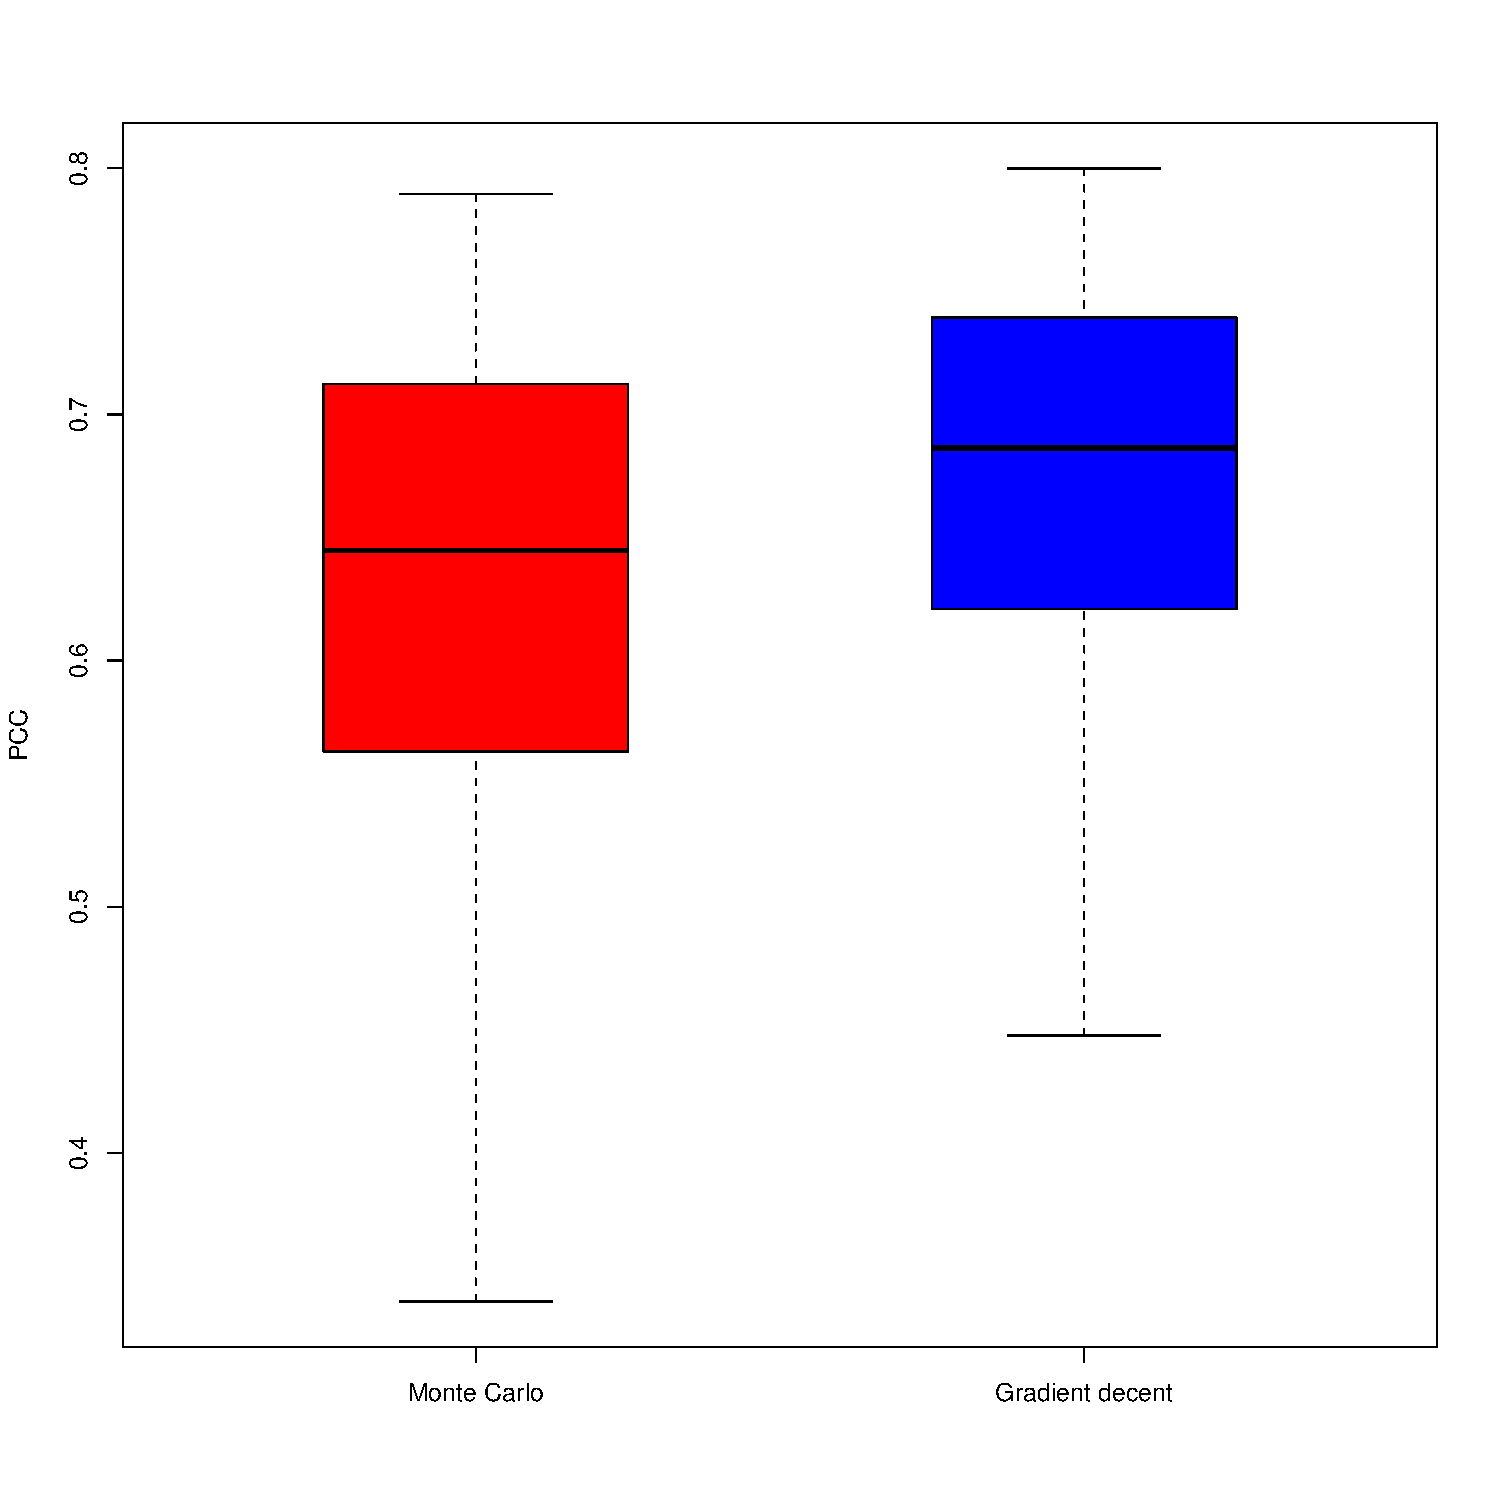
\includegraphics[width=9cm]{fig/boxplot.pdf}}
\caption{Boxplot of the evaluate Pearson correlations obtained with SMM Monte Carlo and Gradient decent at the respective best $\lambda$ values for all the 35 datasets.}
\label{fig:06}
\end{figure}




\par We generally can assume that the gradient decent implementation performs better than the Monte Carlo SMM implementation. 
\par From Figure \ref{fig:06} we can easily see that even if performed with the optimal $\lambda$ value we have lower Pearson correlation coefficients values in the Monte Carlo implementation than in the gradient decent.







%\bibliographystyle{natbib}
%\bibliographystyle{achemnat}
%\bibliographystyle{plainnat}
%\bibliographystyle{abbrv}
%\bibliographystyle{bioinformatics}

\bibliographystyle{abbrv}

\bibliography{algo}


\end{application}
\end{document}
